% Chapter 1

\chapter{Aim and Overview} % Write in your own chapter title
\label{Chapter1}
\lhead{Chapter 1. \emph{Aim and Overview}} % Write in your own chapter title to set the page header

\section{Introduction}

Host genetic factors, including the HLA class I genotype, are major determinants of susceptibility to infectious disease in humans. However, it is currently a difficult task to demonstrate a direct link between the host immune response and the outcome of viral infections in either human or animal populations \citep{Jeffery1999}. Human T-lymphotropic virus-I (HTLV-I) is a persistent retrovirus that infects 10-20 million people worldwide. The virus is endemic in the Caribbean, Japan and parts of Africa. Most infected people remain healthy, but 1-2\% develop a progressive paralytic myelopathy (HTLV-I associated myelopathy/tropical spastic paraparesis; HAM/TSP) and a further 2-3\% develop an aggressive T cell leukaemia/lymphoma. The reasons for these different outcomes is unknown. What is known is that the risk of HAM/TSP is determined, in part, by the host's HLA class I alleles. 

Cells that have become infected with a virus are recognized by the host immune system because they display fragments of the pathogen bound to HLA class I molecules on the infected cell surface. Different people have a diverse range of shapes that make up the HLA class I molecules, owing to their different alleles. Thus, the molecules bind to different parts of the pathogen proteome and present this peptide (or epitope in this context) to CD8$^+$ cytotoxic T lymphocytes (CTLs). Once CTLs recognize the HLA-peptide complex, they are capable of destroying the infected cell by the release of lytic granules containing cytotoxic effector proteins. This results in the destruction of the target cell by apoptosis. An effective CTL response has been shown to confer protection against viral infection, such as HIV \citep{Ngandu2007} and HTLV-I \citep{Bangham2005}. The effectiveness of the response varies between individuals and part of this variation is thought to be due to differences in the host genotype.

The ultimate aim of the project is to increase our understanding of why some HLA class I molecules are better than others at eliciting a more effective immune response. This would increase our knowledge of a key part of the immune system and specifically the design and implementation of improved vaccines.

\section{PhD Design}

\begin{center}
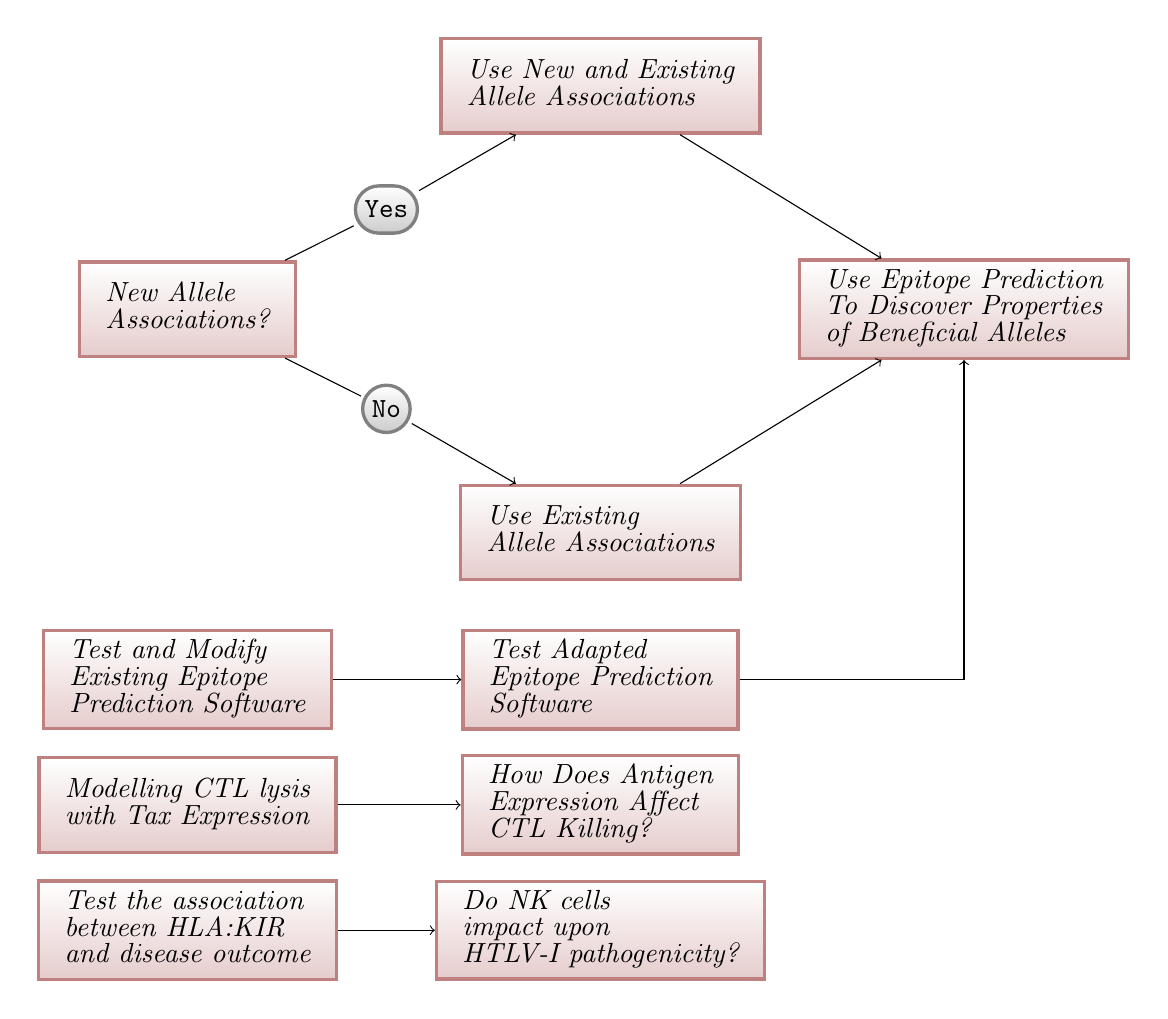
\begin{tikzpicture}[nonterminal/.style={
	rectangle,
	minimum size=12mm,
	very thick,
	draw=red!50!black!50, 
	top color=white, 
	bottom color=red!50!black!20,
	font=\itshape
	},terminal/.style={
	rectangle,minimum size=6mm,rounded corners=3mm,
	very thick,draw=black!50,
	top color=white,bottom color=black!20,
	font=\ttfamily
	},point/.style={
	coordinate,thick,draw=black!50
	}
%	Need to check these with chain	
%	 ,tip/.style={
%	->,shorten >=1pt
%	},every join/.style={
%	rounded corners
%	},hv path/.style={
%	to path={-| (\tikztotarget)}
%	},vh path/.style={
%	to path={|- (\tikztotarget)}
%	}
]

\matrix[row sep=3mm,column sep=2mm] {
% First row
& & \node (atom1) [nonterminal,yshift=9.5mm] {{\renewcommand{\arraystretch}{0.75}\begin{tabular}{l} Use New and Existing \\ Allele Associations \end{tabular}}}; & & \\
& \node (yes1) [terminal] {Yes}; & & & \\
% Second row
\node (atom2) [nonterminal] {{\renewcommand{\arraystretch}{0.75}\begin{tabular}{l} New Allele \\ Associations? \end{tabular}}}; & & & & \node (atom3) [nonterminal] {{\renewcommand{\arraystretch}{0.75}\begin{tabular}{l} Use Epitope Prediction \\ To Discover Properties \\ of Beneficial Alleles \end{tabular}}}; \\
& \node (no1) [terminal] {No}; & & & \\
% Third row
& & \node (atom4) [nonterminal,yshift=-9.5mm] {{\renewcommand{\arraystretch}{0.75}\begin{tabular}{l} Use Existing \\ Allele Associations \end{tabular}}}; & & \\
\\

\node (atom5) [nonterminal] {{\renewcommand{\arraystretch}{0.75}\begin{tabular}{l} Test and Modify \\ Existing Epitope \\ Prediction Software \end{tabular}}}; & & \node (atom6) [nonterminal] {{\renewcommand{\arraystretch}{0.75}\begin{tabular}{l} Test Adapted \\ Epitope Prediction \\ Software \end{tabular}}}; & & \node (pos1) [point] {.};\\
\node (atom7) [nonterminal] {{\renewcommand{\arraystretch}{0.75}\begin{tabular}{l} Modelling CTL lysis \\ with Tax Expression \end{tabular}}}; & & \node (atom8) [nonterminal] {{\renewcommand{\arraystretch}{0.75}\begin{tabular}{l} How Does Antigen \\ Expression Affect \\ CTL Killing? \end{tabular}}}; & & \\
\node (atom9) [nonterminal] {{\renewcommand{\arraystretch}{0.75}\begin{tabular}{l} Test the association \\ between HLA:KIR \\ and disease outcome \end{tabular}}}; & & \node (atom10) [nonterminal] {{\renewcommand{\arraystretch}{0.75}\begin{tabular}{l} Do NK cells \\ impact upon \\ HTLV-I pathogenicity? \end{tabular}}}; & & \\
};

%	chain not working, try again if you have time

\path	(atom2)	edge[-] (yes1)
	(atom2) edge[-] (no1)
	(yes1) 	edge[->] (atom1)
	(no1) 	edge[->] (atom4)
	(atom1) edge[->] (atom3)
	(atom4) edge[->] (atom3);
\path	(atom5) edge[->] (atom6)
	(atom6) edge[-] (pos1)
	(pos1) 	edge[->] (atom3);
\path	(atom7) edge[->] (atom8);
\path	(atom9) edge[->] (atom10);

\end{tikzpicture}
\end{center}

\subsection{Identifying Alleles Associated with Risk or Prevention in HTLV-I Infection}\label{chapter1/AlleleAssoc}

The work of Jeffery \emph{et al.} \citep{Jeffery1999} produced evidence that a number of HLA class I alleles are associated with either disease risk or protection in HTLV-I infection. Added to this, results showing that class I heterozygosity is associated with significantly lower proviral loads \citep{Jeffery2000} would suggest that the protective effect of the HLA haplotype extends to a range of alleles.

Hence, my initial task was to reanalyze a database of individuals from Kagoshima, Japan, who had been infected with HTLV-I and displayed symptoms of HAM/TSP (see \sref{chapter2/HAM/TSP}: HAM/TSP description) or remained asymptomatic. \cref{Chapter3} details the progression of this work.

\subsection{Epitope Prediction}\label{chapter1/EpPred}

There are relatively few experimentally confirmed HTLV-I epitopes for HLA class I alleles compared to HIV. Therefore, in order to test the protective properties of specific HLA class I alleles, it was necessary to use epitope prediction software to predict what epitopes these alleles bind to. The aim of this section was to test the accuracy and predictive power of a number of web-based prediction servers. The starting point was NetCTL v1.2, an integrated web-based prediction method that used information pertaining to proteasomal cleavage, TAP and HLA-peptide binding in epitope prediction. We tested and modified this method, in conjunction with other epitope prediction software, to produce a novel method of epitope prediction that we used for the purpose of discovering the HTLV-I epitopes of ``beneficial'' or ``detrimental'' alleles. The details of this work are in \cref{Chapter4}.

\subsection{The Properties of HLA class I Alleles Associated with Disease Outcome}

Combining the two strands of research, \sref{chapter1/AlleleAssoc} and \sref{chapter1/EpPred}, gave us the ability to predict HTLV-I epitopes for each of the HLA class I alleles contained within the Kagoshima database. Hence, we were able to test what properties of these epitopes were associated with disease risk and proviral load. For instance, we asked the question, ``do alleles associated with protection from disease bind to specific regions of the HTLV-I proteome?''. The details of this work are in \cref{Chapter6}.

\subsection{Modelling CTL Efficiency in Terms of Tax Expression}

In the work detailed above we analyzed the host genetic factors that determine the efficiency of the CD8$^+$ T cell response. We then extended this work to investigate the CD8$^+$ T cell response itself in terms of its properties and dynamics.

In collaboration with experimentalists within the Department of Immunology, we examined the efficiency of CTL-mediated lysis. We tested the hypothesis that the lysis of infected target cells may depend on the expression level of the viral protein Tax in the target cell. This was based on experimental data that showed target cells expressing a higher level of Tax per cell may be killed quicker by CD8$^+$ cells. The analysis consisted of a series of lytic assays, followed by the development of models of Tax expression dynamics and the rate of killing of target cells by CD8$^+$ cells. This data is shown in \cref{Chapter5}.

\subsection{HLA Class I Alleles and KIR Genotype}

One of the main roles of HLA class I molecules is to present antigen to CD8$^+$ T cells. However, HLA-peptide complexes are also recognized by natural killer (NK) cells via their killer cell immunoglobulin (Ig)-like receptors (KIRs). NK cells are critical components of the innate immune system that have direct involvement in the anti-viral immune response. Disease association studies have shown that the interaction between KIR and HLA class I can be protective or detrimental to disease progression in a number of viral infections. In \cref{Chapter7}, we tested the hypothesis that KIR-HLA interactions are predictive of disease status in HTLV-I infection.